\important{Focus sur: la centrale thermique}

\begin{center}
    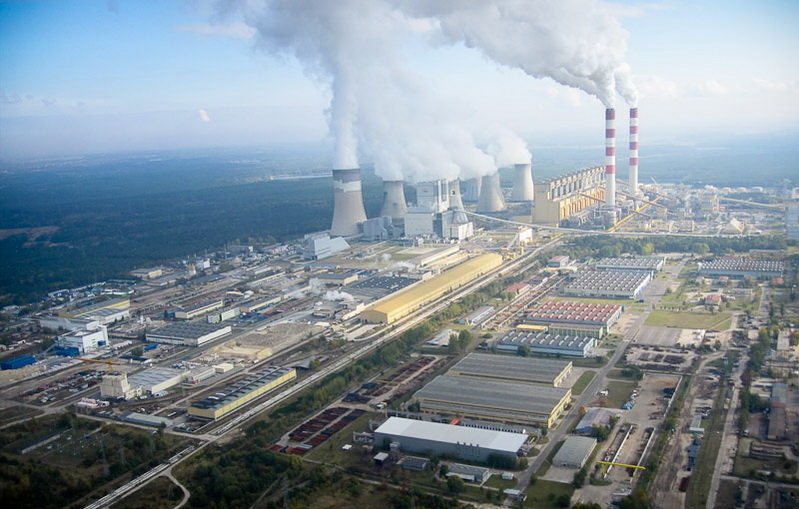
\includegraphics[width=8cm]{images/thermique.jpg}

    \textit{Centrale thermique à charbon de Bełchatów (Pologne)}
\end{center}


Une centrale thermique est un dispositif qui permet de produire de l'électricité à partir d'un combustible fossile : le charbon, le gaz naturel ou le pétrole. Ce combustible est brûlé dans une grande chaudière, ce qui libère beaucoup de chaleur.
Cette chaleur sert à chauffer de l'eau jusqu'à la transformer en vapeur. La vapeur fait alors tourner une turbine, qui entraîne un alternateur produisant de l'électricité.

La centrale thermique utilise des combustibles fossiles, des sources d'énergie non renouvelables, et qui rejettent une grande quantité de CO\textsubscript{2} dans l'atmosphère, contribuant au réchauffement climatique. La combustion produit aussi des fumées qui polluent l'air.
Cependant, sa production est forte et peut être adaptée rapidement à la demande.